\documentclass[10pt,a4paper,twocolumn]{article}
\usepackage[utf8]{inputenc}
\usepackage[T1]{fontenc}
\usepackage[spanish,es-tabla,es-nodecimaldot]{babel}
\usepackage[margin=1.6cm,columnsep=0.6cm]{geometry}
\usepackage{lmodern}
\usepackage{amsmath}
\usepackage{graphicx}
\usepackage{booktabs}
\usepackage{colortbl}
\newcommand{\filasep}{\arrayrulecolor{black!25}\specialrule{0.3pt}{1pt}{1pt}\arrayrulecolor{black}}
\usepackage{tabularx}
\newcolumntype{L}[1]{>{\raggedright\arraybackslash}p{#1}}
\renewcommand{\tabularxcolumn}[1]{>{\raggedright\arraybackslash}p{#1}}
\usepackage{xcolor}
\usepackage{enumitem}
\usepackage{caption}
\usepackage{listings}
\usepackage{fancyhdr}
\usepackage{titlesec}
\usepackage{tikz}
\usetikzlibrary{positioning,arrows.meta,shapes.geometric,calc}
\usepackage[hidelinks]{hyperref}
\setlist{nosep,leftmargin=*}
\captionsetup{font=small,labelfont=bf,skip=3pt}
\setlength{\parskip}{2pt}
\setlength{\parindent}{9pt}
\titleformat{\section}{\large\bfseries}{\thesection}{0.6em}{}
\titlespacing*{\section}{0pt}{7pt}{3pt}
\titleformat{\subsection}{\normalsize\bfseries}{\thesubsection}{0.5em}{}
\titlespacing*{\subsection}{0pt}{5pt}{2pt}
\renewcommand{\floatpagefraction}{0.8}
\setlength{\textfloatsep}{6pt plus 2pt minus 2pt}
\setlength{\floatsep}{5pt plus 2pt minus 2pt}
\setlength{\intextsep}{5pt plus 2pt minus 2pt}

% Marcador (rojo) para datos que el equipo debe completar
\newcommand{\pend}[1]{\textcolor{red}{\textbf{[#1]}}}

\lstset{basicstyle=\ttfamily\tiny,breaklines=true,frame=single,columns=fullflexible}

\pagestyle{fancy}\fancyhf{}
\fancyhead[L]{\small\itshape Portadas infantiles generativas con feedback humano}
\fancyhead[R]{\small\itshape UTEC --- IA}
\fancyfoot[C]{\small\thepage}
\renewcommand{\headrulewidth}{0.4pt}

\begin{document}
\twocolumn[{%
\begin{center}
{\Large\bfseries Sistema Generativo Interactivo de Portadas para Libros Infantiles\\con Parámetros Ajustables, Feedback Humano y Explicación mediante Agentes de IA}\\[3pt]
{\large Proyecto 2 --- Planificación y Toma de Decisiones en IA}\\[4pt]
Andrea Coa \quad Nayeli Guzman \quad Maria Surco \quad Bihonda Epiquien \quad Jimena Gurbillon\\[1pt]
{\small Departamento de Ciencia de la Computación, UTEC \quad Profesora: Dra. Aurea Soriano-Vargas \quad Noviembre 2026}
\end{center}
\vspace{-2pt}
\begin{center}\begin{minipage}{0.92\textwidth}\small
\textbf{Resumen.} Este informe presenta el plan de FROG (\emph{Friendly Rounds Of Generation}, rondas amigables de generación), un sistema que, a partir de un boceto cargado o dibujado por el usuario y de una historia breve que el usuario cuenta, genera exactamente cinco propuestas de portada para un libro infantil. Un agente de historia extrae de la narración los personajes, objetos, lugar y tono (``un conejo que ama las flores'' se convierte en un conejo entre flores) y propone valores para los parámetros, que el usuario confirma. El usuario ajusta parámetros predefinidos (estilo de ilustración, paleta, rango de edad, ambiente, fidelidad al boceto y zona del título) y elige cuál de ellos varía entre las cinco propuestas. Las portadas se generan con dos motores: Stable Diffusion~1.5 con ControlNet (nivel intermedio) y SD-Turbo preentrenado en modo img2img (nivel básico) como respaldo y punto de comparación, ambos gratuitos y ejecutados en Google Colab. Un agente tipográfico elige y acomoda la tipografía del título a partir de un catálogo de fuentes abiertas, el usuario puede cambiarla después, y un renderizador determinista la dibuja para que el título siempre sea correcto y legible. El usuario acepta o rechaza cada propuesta; un planificador basado en muestreo de Thompson usa esas decisiones para proponer la siguiente ronda (máximo tres). Las decisiones se registran en JSON y dos LLM abiertos ejecutados en local (Qwen2.5 y Phi-3.5) redactan resúmenes que un validador determinista contrasta con el registro. Se definen a priori objetivos, restricciones, alcance, métricas, guardrails éticos, plan de evaluación y cronograma.
\end{minipage}\end{center}
\vspace{4pt}
}]

% =====================================================================
\section{Contexto y descripción del problema}
La portada es el primer contacto entre un libro infantil y su lector: es un \emph{paratexto} que anuncia el tono, el género y la edad a la que se dirige la obra antes de que se lea una sola página. En el libro álbum, además, imagen y texto se construyen juntos, por lo que la ilustración de portada condiciona cómo se leerá el título. Que las portadas comunican información visual del contenido lo muestra también que una red convolucional puede predecir el género de un libro solo a partir de su portada.

\textbf{Caso de uso.} Una autora independiente, un docente o un estudiante escribe un cuento infantil (autopublicación, proyecto escolar o concurso). Tiene la historia, por ejemplo ``un conejo que ama las flores y las cuida durante el invierno'', y una idea visual en forma de boceto, pero no cuenta con un ilustrador ni con conocimientos de diseño. Quiere que la portada cuente lo mismo que su historia. Necesita \emph{pocas} propuestas comparables entre sí, entender qué cambia de una a otra y quedarse con un concepto de portada que luego puede refinar o entregar a un ilustrador. Este caso de uso es un supuesto de diseño.

\textbf{Por qué se acota a portadas infantiles.} Acotar el dominio a portadas de libros infantiles permite (i) definir parámetros con significado para el usuario (estilo, paleta, edad), (ii) usar un dataset de referencia del mismo dominio y (iii) concretar los riesgos éticos (contenido apto para niños, imitación de estilos de ilustradores y personajes protegidos).

\textbf{El problema como toma de decisiones.} Los modelos de difusión producen muchas imágenes en segundos, pero esa abundancia traslada el trabajo de elegir al usuario. El problema se puede plantear como \emph{toma de decisiones asistida e iterativa}: elegir entre pocas alternativas y refinar según lo elegido, en la línea de la computación evolutiva interactiva, donde la evaluación subjetiva humana guía la búsqueda, y del aprendizaje automático con humano en el ciclo. Esto plantea cinco dificultades:
\begin{enumerate}
\item \textbf{Control:} las propuestas deben respetar el boceto y la historia y diferir entre sí de forma comparable.
\item \textbf{De la historia a la imagen:} hay que traducir una narración libre en elementos visuales concretos sin inventar lo que la historia no dice, el mismo riesgo de infidelidad que en los resúmenes.
\item \textbf{Texto en la imagen:} los modelos de difusión generan texto ilegible o con errores, y una portada necesita un título correcto, legible y con una tipografía acorde al libro.
\item \textbf{Trazabilidad y planificación:} las decisiones del usuario deben registrarse y reflejarse en cada ronda sin cansarlo con demasiadas iteraciones.
\item \textbf{Explicación fiel:} un LLM que resume puede omitir, inventar o invertir decisiones, y su resumen debe poder verificarse.
\end{enumerate}
\subsection{Definición del problema con design thinking}\label{sec:dt}
Para que el problema parta de las personas y no de la tecnología, la etapa inicial sigue las cinco fases del design thinking: empatizar, definir, idear, prototipar y testear. La Tabla~\ref{tab:dt} resume qué se hace en cada fase y qué produce.

\begin{table}[t]
\centering\scriptsize
\caption{Fases de design thinking aplicadas al proyecto.}\label{tab:dt}
\begin{tabularx}{\columnwidth}{@{}L{1.25cm}XL{1.75cm}@{}}
\toprule
\textbf{Fase} & \textbf{Actividad} & \textbf{Producto}\\
\midrule
Empatizar & Entrevistas semiestructuradas de 20--30\,min a 5 personas: 2 docentes de inicial o primaria, 2 personas que escriben cuentos (estudiantes o autores independientes) y 1 ilustrador o diseñador. Preguntas: cómo consiguen hoy una portada, qué les frustra, cómo describen lo que quieren y qué esperan de una herramienta con IA & Mapa de empatía\\
\filasep
Definir & Síntesis de las entrevistas en una proto-persona, un punto de vista (POV) y una pregunta ``¿Cómo podríamos...?'' & POV y requisitos\\
\filasep
Idear & Lluvia de ideas del equipo y matriz impacto--esfuerzo para elegir qué entra en el alcance & Ideas priorizadas\\
\filasep
Prototipar & Prototipo en papel de la interfaz y un cuaderno de Colab que genera una ronda con un boceto & Prototipos\\
\filasep
Testear & Prueba piloto con 2 usuarios (semana 3) y estudio E4 con 10 participantes & Ajustes al diseño\\
\bottomrule
\end{tabularx}
\end{table}

\textbf{Proto-persona (supuesto inicial).} \emph{Carmen, 34 años, docente de inicial.} Escribe cuentos cortos para su aula y quiere imprimir algunos como libritos para sus alumnos. Sabe lo que quiere contar y hace dibujos simples, pero no sabe diseñar, no puede pagar un ilustrador por cada cuento y las herramientas de IA que probó le dieron imágenes que no se parecían a su idea ni a su historia, con el título mal escrito. Esta persona es una hipótesis construida antes de las entrevistas; se ajustará con sus hallazgos \pend{hallazgos de las entrevistas}.

\textbf{Mapa de empatía y propuesta de valor (supuestos).} Antes de entrevistar, el equipo registró sus supuestos sobre Carmen en un mapa de empatía y en un lienzo de propuesta de valor (Tabla~\ref{tab:empatia}). Tras las entrevistas se hace un mapa por participante y se compara con este para ver qué supuestos se confirman. En el lienzo, cada aliviador de FROG responde a una frustración (no hace falta dibujar bien, no hay marcas de agua ni pagos, el título se verifica con OCR y el contenido se filtra para niños) y cada creador de alegrías a una ganancia esperada (respetar el boceto, usar la historia y aprender de las decisiones en hasta tres rondas).

\begin{table}[t]
\centering\scriptsize
\caption{Mapa de empatía de la proto-persona (supuestos previos a las entrevistas).}\label{tab:empatia}
\begin{tabularx}{\columnwidth}{@{}L{1.3cm}X@{}}
\toprule
\textbf{Cuadrante} & \textbf{Supuestos}\\
\midrule
Dice & ``Me gusta escribir libros, pero soy mala dibujando''; ``le pongo fotos con marca de agua''\\
\filasep
Piensa & ``Quisiera que mis niños tuvieran libros con dibujos''; ``¿y si la IA no entiende mi cuento?''\\
\filasep
Hace & Hace la portada sin dibujo o usa imágenes genéricas que no representan su cuento\\
\filasep
Siente & Tristeza, conformismo, desmotivación\\
\filasep
Dolores & No puede pagar un ilustrador; la IA ignora su idea y escribe mal los títulos; poco tiempo\\
\filasep
Ganancias & Una portada que se parezca a su cuento, a partir de su dibujo, gratis y eligiendo entre opciones\\
\bottomrule
\end{tabularx}
\end{table}

\textbf{Punto de vista.} Carmen \emph{necesita} obtener rápido unas pocas portadas que respeten su dibujo y cuenten su historia, y poder elegir entre ellas, \emph{porque} sabe reconocer lo que quiere al verlo aunque no sepa diseñarlo, y las herramientas genéricas le dan resultados que no controla.

\textbf{Pregunta guía.} \emph{¿Cómo podríamos} ayudar a quien escribe un cuento infantil a convertir su boceto y su historia en una portada que reconozca como suya, decidiendo entre pocas opciones claras y entendiendo por qué el sistema le propone cada una?

\textbf{De la fase de ideación al alcance.} De las ideas evaluadas, entraron al alcance las de mayor impacto y esfuerzo razonable: partir del boceto, usar la historia, ofrecer parámetros con nombres comprensibles, componer el título aparte y aprender de las decisiones entre rondas. Quedaron fuera, por esfuerzo alto o por salir del enunciado, generar sin boceto, procesar libros completos, diseñar contraportada y lomo, y editar regiones de la imagen con pincel.
% =====================================================================
\section{Objetivos}
\subsection{Objetivo general}
Desarrollar un sistema generativo interactivo que proponga portadas para libros infantiles a partir de un boceto y una historia, y que incorpore las decisiones del usuario en cada ronda.

\subsection{Objetivos específicos}
\begin{enumerate}
\item \textbf{Datos:} analizar un dataset de portadas infantiles reales para obtener rangos de referencia (color, brillo, densidad visual, zona del título) y preparar un conjunto de bocetos de prueba.
\item \textbf{Generación:} implementar dos motores (SD~1.5 con ControlNet, nivel intermedio, y SD-Turbo en modo img2img, nivel básico) que produzcan cinco propuestas controladas por parámetros, con un agente que extraiga los elementos de la historia y otro que componga el título.
\item \textbf{Interacción y planificación:} construir una interfaz para aceptar o rechazar cada propuesta indicando el motivo, y un planificador que use esas decisiones en la ronda siguiente.
\item \textbf{Explicación:} integrar dos LLM que resuman las decisiones, con un validador que contraste cada resumen con el registro.
\item \textbf{Evaluación y ética:} medir la calidad, la seguridad, el efecto del planificador y la usabilidad, e implementar guardrails para contenido apto para niños.
\end{enumerate}

% =====================================================================
\section{Restricciones}
\textbf{De cómputo.} El motor local debe ejecutarse en una GPU de 16\,GB (NVIDIA T4 de Google Colab). La meta de diseño es generar una ronda de cinco propuestas en menos de 60\,s. Todos los modelos son de código abierto y se ejecutan en Colab, sin APIs externas.

\textbf{Del enunciado.} Exactamente cinco variaciones por imagen de entrada; dos de los tres niveles de implementación; una interfaz gráfica que registre aceptación o rechazo; un agente LLM que indique explícitamente qué se aceptó y qué se rechazó; y un informe de máximo diez páginas.

\textbf{De diseño.} La entrada es un boceto o dibujo (no fotografías de personas) más una historia de hasta 500 palabras; el boceto es obligatorio porque el enunciado exige una imagen de entrada, y la historia lo complementa; el formato de salida es vertical 2:3 (512$\times$768\,px), proporción habitual de tapa; se hacen como máximo tres rondas por sesión; no se entrena ni ajusta ningún modelo; los agentes nunca reciben imágenes: el de historia recibe el texto, el tipográfico recibe medidas calculadas de la portada y el explicador recibe el registro JSON.

\textbf{Normativas y éticas.} El contenido debe ser apto para niños; no se procesan fotografías de menores; no se imitan estilos de ilustradores con nombre propio ni personajes protegidos; las portadas del dataset se usan solo para análisis estadístico y no se redistribuyen; las imágenes del usuario no se guardan fuera de la sesión.

% =====================================================================
\section{Alcance}
\textbf{Incluye:} un boceto, una historia breve y un título por sesión; extracción de elementos de la historia; cinco parámetros predefinidos con cinco valores cada uno (más la zona del título como ajuste fijo), además de una instrucción libre filtrada; tipografía elegida por un agente y editable por el usuario; cinco propuestas por ronda y hasta tres rondas; dos motores de generación; composición determinista del título; registro de decisiones; resumen verificado con dos LLM; guardrails de entrada y de salida; evaluación automática sobre bocetos de prueba, una simulación del planificador y un estudio de usabilidad pequeño.

\textbf{No incluye:} contraportada, lomo ni archivo de imprenta (sangrado, CMYK); ilustraciones interiores; procesar libros completos (solo una historia o sinopsis breve); generar sin boceto; entrenamiento o ajuste fino; aprendizaje de preferencias entre sesiones; uso comercial; ni garantías sobre la protección por derechos de autor de la portada resultante. El resultado se presenta como \emph{concepto de portada}, no como arte final.

% =====================================================================
\section{Diseño del sistema y arquitectura}\label{sec:arq}
La Figura~\ref{fig:arq} muestra el flujo de información y los puntos de decisión. El sistema tiene siete módulos:
(1)~\textbf{preprocesamiento, guardrails de entrada y agente de historia};
(2)~\textbf{planificador}, que decide las cinco configuraciones de la ronda;
(3)~\textbf{motores generativos} A y B;
(4)~\textbf{guardrails de salida y agente tipográfico}, que acomoda el título;
(5)~\textbf{interfaz} de evaluación;
(6)~\textbf{registro} JSON; y
(7)~\textbf{agente explicador} con validador.
El usuario puede pedir otra ronda (como máximo tres), y el resumen se habilita cuando las cinco tarjetas de la última ronda tienen una decisión.

\begin{figure*}[!t]
\centering
\begin{tikzpicture}[
  font=\scriptsize,
  node distance=5mm and 3.5mm,
  box/.style={draw, rounded corners=2pt, align=center, minimum height=11mm, text width=27mm, fill=#1},
  box/.default=gray!8,
  dec/.style={draw, diamond, aspect=2, align=center, inner sep=0.5pt, fill=orange!15, text width=17mm},
  arr/.style={-{Latex[length=1.8mm]}, semithick},
  lbl/.style={font=\tiny, fill=white, inner sep=1pt}]
\node[box=blue!8] (in) {\textbf{Usuario}\\boceto + historia +\\título + parámetros};
\node[box, right=of in] (pre) {\textbf{1} Preprocesamiento\\+ guardrails de entrada\\+ agente de historia};
\node[box=yellow!18, right=of pre] (plan) {\textbf{2} Planificador\\5 configuraciones\\(Thompson, Beta)};
\node[box=green!12, right=of plan] (gen) {\textbf{3} Motor A: SD 1.5 +\\ControlNet\\Motor B: SD-Turbo};
\node[box, right=of gen] (post) {\textbf{4} Guardrails de salida\\+ agente tipográfico\\+ render del título};
\node[box=blue!8, below=10mm of post] (ui) {\textbf{5} Interfaz Gradio\\aceptar / rechazar\\+ motivo\\+ editar fuente};
\node[box=yellow!18, left=of ui] (log) {\textbf{6} Registro JSON\\parámetros, semillas,\\decisiones, motivos};
\node[dec, left=of log] (more) {¿Otra ronda?\\($r<3$)};
\node[box=violet!12, left=of more] (llm) {\textbf{7} Agente LLM\\Qwen2.5 | Phi-3.5\\resumen + JSON};
\node[dec, left=of llm] (val) {¿Coincide con\\el registro?};
\node[box=blue!8, below=6mm of val] (res) {Resumen final\\al usuario};
\node[box, below=6mm of llm] (tpl) {Resumen por\\plantilla (respaldo)};
\draw[arr] (in) -- (pre);
\draw[arr] (pre) -- (plan);
\draw[arr] (plan) -- (gen);
\draw[arr] (gen) -- (post);
\draw[arr] (post) -- (ui);
\draw[arr] (ui) -- (log);
\draw[arr] (log) -- (more);
\draw[arr] (more.north) -- node[lbl, right]{sí: actualizar preferencias} (more.north |- plan.south);
\draw[arr] (more) -- node[lbl, above]{no} (llm);
\draw[arr] (llm) -- (val);
\draw[arr] (val) -- node[lbl, right]{sí} (res);
\draw[arr] (val.north) -- ++(0,3mm) -| node[lbl, pos=0.25, above]{no: reintento (máx.\ 2)} (llm.north);
\draw[arr] (llm) -- node[lbl, right]{si fallan los reintentos} (tpl);
\draw[arr] (tpl) -- (res);
\draw[arr, dashed] (pre.north) -- ++(0,3mm) node[lbl, above]{rechazo: boceto vacío, rostro real o contenido no apto};
\draw[arr, dashed] ([xshift=8mm]ui.north) -- node[lbl, right]{cambio de fuente} ([xshift=8mm]post.south);
\end{tikzpicture}
\caption{Arquitectura y flujo de decisiones. Los rombos son puntos de decisión; la flecha punteada indica el rechazo de la entrada por los guardrails.}\label{fig:arq}
\end{figure*}

\subsection{Parámetros ajustables y eje de variación}
El agente de historia propone valores iniciales para la edad, el ambiente y la escena; el usuario los confirma o corrige, fija el resto de los parámetros (Tabla~\ref{tab:param}) y elige uno como \textbf{eje de variación}: las cinco propuestas toman los cinco valores de ese parámetro y comparten el resto. Así cada propuesta difiere en un atributo conocido, lo que facilita compararlas y atribuir la decisión del usuario a ese atributo. Se ofrecen tres modos:
\begin{itemize}
\item \textbf{Paquete de exploración} (por defecto): el eje es el estilo, para ver primero cinco estilos distintos.
\item \textbf{Individual:} el usuario elige el eje (p.\,ej., cinco paletas con un estilo ya elegido).
\item \textbf{Libre:} el usuario añade una instrucción escrita (p.\,ej., ``un zorro leyendo bajo un árbol''), que pasa por el filtro de la Sección~\ref{sec:etica} y se agrega a las cinco propuestas.
\end{itemize}

\begin{table}[t]
\centering\scriptsize
\caption{Parámetros ajustables y su traducción al prompt (valores iniciales, se ajustarán en la calibración).}\label{tab:param}
\begin{tabularx}{\columnwidth}{@{}L{1.45cm}X@{}}
\toprule
\textbf{Parámetro} & \textbf{Valores (fragmento de prompt o ajuste técnico)}\\
\midrule
Estilo & acuarela (\textit{watercolor}); lápices de colores (\textit{colored pencil, crayon}); collage de papel (\textit{cut paper collage}); vectorial plano (\textit{flat vector}); plastilina 3D (\textit{clay 3D render})\\
\filasep
Paleta & pastel; cálida; fría; primarios vivos; tierra (prompt y rango objetivo de tono, saturación y brillo)\\
\filasep
Edad & 0--3 (formas muy simples, alto contraste, un solo personaje); 4--6; 7--9 (más detalle y fondo); 10--12; sin indicar\\
\filasep
Ambiente & alegre; aventura; calma o para dormir; misterio suave; humor\\
\filasep
Fidelidad & muy baja a muy alta: escala de ControlNet 0.6--0.8 (motor A); no aplica al motor~B\\
\filasep
Zona del título & ajuste fijo (superior por defecto; el usuario puede cambiarla, pero no se varía entre propuestas): superior; inferior; superior e inferior; centrada; sin título\\
\filasep
Tipografía & no la elige el usuario al inicio: la propone el agente tipográfico (fuente del catálogo, curva, onda, inclinación de letras, contorno, color) y el usuario puede cambiarla en cada tarjeta\\
\bottomrule
\end{tabularx}
\end{table}

La relación entre paleta y ambiente se apoya, como hipótesis de diseño, en que los niños asocian los colores brillantes con emociones positivas y los oscuros con negativas; ese estudio se hizo con 60 niños de 5 y 6 años, por lo que no se asume que el efecto se generalice y solo se usa para elegir valores por defecto. Las reglas por edad son supuestos de diseño que se contrastarán con los participantes.

\subsection{Decisiones técnicas}
\textbf{Dos motores (niveles intermedio y básico).} El enunciado pide implementar dos de los tres niveles. El \textbf{motor~A} (intermedio, principal) usa un modelo de difusión latente preentrenado condicionado con ControlNet, que fija la estructura del boceto y deja libres color, textura y estilo. El \textbf{motor~B} (básico) usa SD-Turbo, un modelo preentrenado destilado para generar en uno a cuatro pasos, en modo img2img: parte del mismo boceto y del mismo prompt, sin control estructural adicional. Se considera nivel básico porque solo reutiliza un modelo preentrenado sin condicionarlo con módulos adicionales, a diferencia del motor~A. Ambos modelos se descargan de Hugging Face y se ejecutan en la GPU de la sesión de Colab; no se consume ninguna API externa. B sirve como respaldo rápido si el motor A se queda sin memoria y como línea base: al no tener ControlNet, permite medir cuánto aporta el control al respeto del boceto. El usuario puede elegir el motor en la interfaz. Se descarta el nivel avanzado (entrenar una GAN o un modelo propio) por el costo de cómputo y de datos.

\textbf{Agente de historia.} El usuario cuenta su historia en un campo de texto (hasta 500 palabras). Un LLM con temperatura 0 la convierte en un JSON con personajes, objetos, lugar, momento del día, tono y edad sugerida; por ejemplo, ``un conejo que ama las flores'' da \lstinline[basicstyle=\ttfamily\footnotesize]|{"personajes":["conejo"],"objetos":["flores"],"lugar":"jardin"}|. Estos elementos forman la parte de escena del prompt y proponen la edad y el ambiente. Para no inventar lo que la historia no dice, un verificador comprueba que cada personaje y objeto aparezca en el texto (coincidencia de lemas o sinónimo de una lista corta) y marca los que no; la interfaz muestra la lista y el usuario la confirma o edita antes de generar. El agente no añade género, etnia ni rasgos físicos que la historia no mencione. Como un manuscrito inédito es información valiosa para su autor, la historia se procesa solo con modelos que corren en la misma sesión de Colab: el texto nunca se envía a un servicio externo.

\textbf{Agente tipográfico y título fuera del modelo.} Como la difusión genera texto poco fiable, el prompt negativo excluye texto y letras, y el título se añade después. El usuario no elige la fuente al inicio: un agente tipográfico (el mismo LLM local, con temperatura 0) la propone a partir de medidas calculadas sobre cada portada (cantidad de trazo, brillo, color medio y colores dominantes de la zona del título y el contraste que daría un texto oscuro o uno claro), del estilo y ambiente elegidos, de la edad y de la longitud del título. Devuelve un JSON con valores de un espacio acotado: fuente de un catálogo de cuatro familias con licencia SIL OFL, cuyos textos de licencia se incluyen en el repositorio (Andika, diseñada para lectores principiantes, Fredoka, Baloo~2 y Lilita One), tamaño, curva del arco, onda, inclinación por letra, contorno y color. Un renderizador determinista con Pillow aplica esos valores letra por letra y los recorta a sus límites (p.\,ej., curva e inclinación máximas; para lectores de 0 a 6 años solo Andika o Fredoka, con poca inclinación y onda), de modo que el agente puede ``deformar'' el título de forma lúdica pero nunca escribir mal una letra. El color se ajusta para alcanzar un contraste de al menos 4.5:1 con el fondo, el criterio WCAG~2.1 para texto normal; si no se logra, se añade una banda semitransparente. En cada tarjeta, el usuario puede cambiar fuente, curva, tamaño y color; el cambio solo vuelve a renderizar el título (no regenera la imagen) y queda registrado como retroalimentación. Si el agente falla o devuelve valores no válidos tras un reintento, se usa una disposición por defecto según la edad.

\textbf{Planificación con muestreo de Thompson.} Para que las iteraciones reflejen las decisiones, cada valor $v$ de cada parámetro $p$ tiene una distribución $\mathrm{Beta}(\alpha_{p,v},\beta_{p,v})$, con $\alpha=\beta=1$ al inicio. Sea $V$ el conjunto de parámetros que variaron entre las cinco propuestas de la ronda (un parámetro igual en las cinco no informa sobre la preferencia y no se actualiza). Al cerrar la ronda:
\begin{equation}
\begin{aligned}
\text{aceptada } i &: \ \alpha_{p,v_i(p)} \mathrel{+}= 1 \quad \forall p\in V,\\
\text{rechazada } i &: \ \beta_{p,v_i(p)} \mathrel{+}= 1 \quad \forall p\in M_i\cap V,
\end{aligned}
\end{equation}
donde $M_i$ son los parámetros marcados como motivo del rechazo (\emph{estilo}, \emph{colores}, \emph{no apto para la edad}, \emph{ambiente}, \emph{se aleja del boceto}). Si no queda ninguno (no se marcó motivo o este se refiere a un parámetro que no varió), se penaliza solo el eje de la ronda. En la ronda siguiente el usuario elige un nuevo eje; para cada una de las cinco propuestas, los demás parámetros no fijados se obtienen por muestreo de Thompson, es decir, tomando el valor con mayor muestra $\theta_{p,v}\sim\mathrm{Beta}(\alpha_{p,v},\beta_{p,v})$. Así se explota lo aceptado sin dejar de explorar. Las semillas cambian en cada ronda. El límite de tres rondas responde a la fatiga del usuario, una limitación conocida de la evaluación humana interactiva.

% =====================================================================
\section{Selección y preparación de datos}\label{sec:datos}
Como los modelos son preentrenados, los datos no se usan para entrenar sino para (a) caracterizar el dominio, (b) simular entradas de usuario en la evaluación automática y (c) servir de distribución de referencia.

\textbf{D1: portadas reales (referencia).} \emph{Book Cover Dataset}: el listado Book32 tiene 207\,572 libros de Amazon en 32 categorías, con enlace a la portada, título y autor; se usa la categoría \emph{Children's Books}, con 13\,605 libros. Se elige porque es un dataset académico de portadas con etiqueta de género. Las portadas tienen derechos de autor, por lo que se usan solo para estadísticas y como referencia del KID, sin redistribuirlas ni usarlas para entrenar. Se tomó una muestra aleatoria de 2\,000 portadas; aunque los enlaces son de 2016, todas siguen disponibles tras actualizar el dominio de las imágenes.

\textbf{D2: bocetos simulados (entrada).} \emph{Quick, Draw!}: más de 50 millones de dibujos de trazos hechos en menos de 20\,s, publicados bajo CC BY 4.0. Se eligen 10 categorías propias de cuentos infantiles (gato, perro, conejo, oso, pez, pájaro, árbol, casa, sol y dragón) y 20 dibujos por categoría, $N=200$ entradas.

\textbf{D3: bocetos realistas.} Alrededor de 20 bocetos hechos a mano por el equipo, fotografiados con celular, para probar casos más cercanos al uso real (sombras, papel con textura, trazos irregulares) y para la demostración.

\textbf{D4: historias de prueba.} \emph{TinyStories}: cuentos breves sintéticos escritos con vocabulario de niños de 3 a 4 años, publicados bajo licencia CDLA-Sharing-1.0. Se seleccionaron 200 historias cuyo personaje principal pertenezca a una de las 10 categorías de D2, y cada una se emparejará con un boceto de su categoría. Las historias se usan en inglés, su idioma original: una prueba de traducción automática con MarianMT produjo errores (nombres propios traducidos, cambios de género) que habrían contaminado la referencia. Además se anotarán a mano los elementos visuales de 30 historias, que servirán como referencia para evaluar al agente de historia.

\textbf{D4-es.} Para evaluar al agente en el idioma de la aplicación se descargaron con la API de Wikisource 250 cuentos y fábulas en español de dominio público; tras quitar 41 por el filtro de contenido y 12 por longitud, se eligieron 60 en prosa (48 de Godofredo Daireaux, 3 de Horacio Quiroga, 9 de Esopo y Fedro), de las que se anotarán 30.

\textbf{Análisis exploratorio.} Sobre D1 se midieron colorido, brillo, saturación, proporción de tonos cálidos, fríos y tierra, paletas dominantes (k-means en CIELAB, $k=5$), densidad de bordes por tercio vertical y posición del título con OCR. Las portadas infantiles son claras y moderadamente saturadas (medianas: brillo 0.70, saturación 0.39, colorido 72 con rango intercuartílico 53--94), y predominan los tonos cálidos (43\,\% de los píxeles con color, frente a 18\,\% fríos). El título está en el tercio superior en el 72\,\% de las portadas (17\,\% en el medio y 10\,\% abajo), y ese tercio es el de menor densidad de bordes (mediana 0.087 frente a 0.097 y 0.095): esto respalda la zona superior como valor por defecto, y el percentil 75 de esa densidad (0.111) es el umbral de la Tabla~\ref{tab:met}. Los criterios de paleta se fijaron en el cuartil más característico de cada rasgo, de modo que cada paleta abarca entre el 18 y el 29\,\% de las portadas reales. Dos hallazgos limitan el diseño: la mediana de la proporción alto/ancho es 1.28 y una de cada cuatro portadas es casi cuadrada, más baja que nuestro formato 2:3 (1.5); y la categoría \emph{Children's Books} incluye no ficción para lectores mayores, así que la referencia es más amplia que los cuentos ilustrados. En D2 la tinta va de 1.5 a 10.6\,\% (mediana 5.3\,\%) y el contenido ocupa en mediana el 67\,\% del lienzo, dentro de los umbrales de validación, por lo que ningún boceto se rechaza por error.

\textbf{Preprocesamiento de la entrada.}
(1)~Eliminación de metadatos EXIF y conversión a escala de grises;
(2)~para fotos de dibujos, extracción de líneas con HED; para bocetos limpios, binarización de Otsu;
(3)~validación: se rechaza un boceto vacío (tinta $<0.5$\,\%) o saturado (tinta $>40$\,\%, umbrales iniciales);
(4)~recorte al contenido y ubicación en un lienzo 2:3 dejando libre la zona del título elegida;
(5)~redimensionado a 512$\times$768 (múltiplo de 8 requerido por el VAE);
(6)~para D2, rasterizado de los trazos con un grosor de 6\,px.
Si el usuario sube una foto en color de un dibujo, se ofrece además el modo img2img para conservar sus colores.

\subsection{Propiedad intelectual y licencias}\label{sec:pi}
Cada recurso tiene dueño y condiciones de uso distintas, así que se revisó la licencia de cada uno antes de incluirlo (Tabla~\ref{tab:pi}). Se distinguen tres casos.

\textbf{Datos con derechos reservados (D1).} Las portadas de Amazon son obras protegidas de sus ilustradores y editoriales; el dataset distribuye enlaces y metadatos, no una licencia sobre las imágenes. En el Perú, la Ley sobre el Derecho de Autor no tiene una cláusula general como el \emph{fair use} estadounidense, sino una lista de usos permitidos sin autorización, como la cita (art.~44). Por eso se adopta el uso más conservador: las portadas se descargan solo para calcular estadísticas y la referencia del KID, no se muestran en el informe ni en la demo, no se redistribuyen y no se usan para entrenar.

\textbf{Datos con licencia abierta (D2, D4, tipografías).} Quick, Draw! (CC BY 4.0) obliga a citar la fuente. TinyStories (CDLA-Sharing-1.0) permite usar y modificar los datos, pero si se publican datos derivados deben compartirse con la misma licencia; aquí se usan sin modificar. Las tipografías OFL pueden incluirse en el software, pero no venderse por separado.

\textbf{Modelos y salidas.} Stable Diffusion~1.5 se publica bajo CreativeML OpenRAIL-M, que permite usarlo pero prohíbe una lista de usos dañinos y obliga a mantener esas restricciones si se redistribuye; ControlNet~1.1 usa una licencia de la misma familia. SD-Turbo usa la Stability AI Community License, que permite el uso académico. Qwen2.5-7B-Instruct usa Apache~2.0 y Phi-3.5-mini-instruct, MIT. Sobre las portadas generadas, la ley peruana reconoce como autor a la persona natural que crea la obra, y la Oficina de Derechos de Autor de EE.\,UU. concluye que lo generado por IA solo se protege en la medida de la contribución humana perceptible. Por eso el sistema registra la contribución del usuario (boceto, historia, decisiones y ediciones) y le advierte que su protección no está garantizada. El boceto y la historia siguen siendo del usuario: no se almacenan ni se usan para otro fin. Este análisis es académico y no sustituye una asesoría legal.

\begin{table}[t]
\centering\scriptsize
\caption{Recursos, licencia y uso que se les da en el proyecto.}\label{tab:pi}
\begin{tabularx}{\columnwidth}{@{}L{1.6cm}L{1.7cm}X@{}}
\toprule
\textbf{Recurso} & \textbf{Licencia} & \textbf{Uso en el proyecto}\\
\midrule
D1 portadas & Derechos reservados & Solo estadísticas y referencia; sin mostrar, redistribuir ni entrenar\\
\filasep
D2 Quick, Draw! & CC BY 4.0 & Entradas de prueba; se cita la fuente\\
\filasep
D3 bocetos propios & Del equipo & Pruebas y demo, con consentimiento de quien dibuja\\
\filasep
D4 TinyStories & CDLA-Sharing-1.0 & Historias de prueba, en inglés y sin modificar\\
\filasep
D4-es Wikisource & Dominio público & Historias de prueba en español; se guarda la URL de cada una\\
\filasep
SD 1.5, ControlNet & OpenRAIL-M & Generación respetando los usos prohibidos\\
\filasep
SD-Turbo & Stability AI Community License & Motor B\\
\filasep
Qwen2.5-7B, Phi-3.5-mini & Apache 2.0, MIT & Agentes en local\\
\filasep
Andika, Fredoka, Baloo 2, Lilita One & SIL OFL 1.1 & Título de la portada\\
\filasep
Boceto e historia del usuario & Del usuario & Solo durante la sesión; se guarda el hash\\
\bottomrule
\end{tabularx}
\end{table}

% =====================================================================
\section{Modelo generativo}
\textbf{Motor A.} \texttt{stable-diffusion-v1-5} con \texttt{control\_v11p\_sd15\_scribble} para bocetos y \texttt{control\_v11p\_sd15\_lineart} para dibujos con líneas limpias (ControlNet~1.1), en la biblioteca \texttt{diffusers}, con media precisión (fp16) y \emph{attention slicing} para la T4. Planificador DPM-Solver++ con 25 pasos y escala de guía 7.0. Las cinco imágenes se generan en un solo lote con semillas fijas y registradas. Los parámetros se traducen al prompt con la plantilla de la Figura~\ref{fig:prompt}, que pone primero lo más importante porque CLIP solo lee 77 tokens.

\begin{figure}[t]
\begin{lstlisting}
prompt: "{estilo}, children's picture book cover illustration,
  {escena: a rabbit among flowers in a garden}, {paleta}, {ambiente},
  {complejidad por edad}, {zona del titulo: empty space at the top},
  {instruccion libre}"
negativo: "text, letters, words, watermark, signature, scary, violent,
  blood, weapon, nsfw, deformed, extra limbs, lowres"
\end{lstlisting}
\caption{Plantilla de prompt y prompt negativo comunes a los dos motores.}\label{fig:prompt}
\end{figure}
\textbf{Experimento con LoRA.} El enunciado sugiere explorar modelos de Hugging Face y Civitai. Se probó el adaptador LoRA \texttt{alvdansen/dimension-w-sd15}, cuya ficha indica licencia CreativeML OpenRAIL-M y base SD~1.5, sin nombrar a un artista, pero sin documentar sus datos de entrenamiento (una limitación que se reporta). Con 20 bocetos y escalas 0, 0.6 y 1.0, el CLIPScore sube de 0.72 a 0.74 y 0.76, pero el acierto de estilo baja de 95 a 75 y 45\,\%: el adaptador impone su propio estilo y pisa el parámetro que el usuario elige, así que no se incorpora al sistema.

\textbf{Motor B.} \texttt{stabilityai/sd-turbo} con \texttt{AutoPipelineForImage2Image}, 10 pasos, \texttt{strength}~=~0.90 y sin guía (\texttt{guidance\_scale}~=~0, por lo que no usa el prompt negativo; los guardrails de salida compensan). Un barrido de \texttt{strength} (0.7--0.95) y de pasos (4--20) mostró que SD-Turbo no tiene un punto intermedio fiable: o copia el boceto o lo reemplaza. Por eso el motor B reinterpreta el dibujo con libertad (conserva la categoría, no la pose) y la fidelidad no se ajusta en este motor. Se usa si el motor A se queda sin memoria o si el usuario lo elige; al ser mucho más rápido, se evalúa con los mismos 200 pares que el motor A.

\textbf{Calibración.} Con 20 bocetos de D2 se barrió la escala de ControlNet $\in\{0.4,0.6,\dots,1.4\}$ y los pasos $\in\{20,25,30\}$, midiendo la cobertura de los bordes del boceto (\emph{recall}) y el acierto de estilo. Con 20 pasos, el recall pasa de 0.15 (escala 0.4) a 0.25--0.26 entre 0.6 y 1.0 y vuelve a bajar a 0.19 en 1.4, mientras que el acierto de estilo se mantiene en 90--95\,\% hasta 0.8 y cae a 80--85\,\% desde 1.0. Los pasos 25 y 30 no mejoran el resultado, así que se usan 20 pasos y los cinco valores de fidelidad van de 0.60 a 0.80 en pasos de 0.05, la zona en que ambas métricas son buenas.

% =====================================================================
\section{Interfaz e interacción humano--IA}
La interacción sigue pautas de interacción humano--IA: mostrar qué cambia cada opción, permitir corregir decisiones y explicar el comportamiento del sistema. La interfaz se construye con \texttt{gradio.Blocks}:
\begin{enumerate}
\item \textbf{Entrada:} subir una imagen o dibujar en un lienzo (\texttt{gr.Sketchpad}); contar la historia; escribir título, autor y, si se desea, una instrucción libre; declarar que el boceto es propio o que se cuenta con permiso (si lo dibujó un menor, con permiso de su tutor).
\item \textbf{Escena:} lista editable de los elementos que el agente extrajo de la historia (los no encontrados en el texto aparecen marcados), que el usuario confirma.
\item \textbf{Parámetros:} menús con los valores de la Tabla~\ref{tab:param} (con los propuestos por el agente ya seleccionados), selección del eje, del modo y del motor.
\item \textbf{Propuestas:} cinco tarjetas con la portada ya titulada, una etiqueta con el valor que cambia (``Paleta: pastel'') y botones \emph{Aceptar} y \emph{Rechazar}; al rechazar se muestran casillas de motivo y un comentario opcional. Un botón ``Editar título'' abre los controles de fuente, tamaño, curva y color, con vista previa inmediata. Hay además un botón ``Aceptar o rechazar todo'' para dar retroalimentación por paquete.
\item \textbf{Rondas:} ``Nueva ronda'' (si $r<3$) muestra qué cambiará el planificador antes de generar; ``Generar resumen'' se habilita cuando las cinco tarjetas tienen decisión, que puede cambiarse hasta ese momento.
\item \textbf{Salida:} descarga en PNG de las portadas aceptadas, con la marca ``Generado con IA'' en los metadatos.
\end{enumerate}
Cada sesión se guarda en un JSON:
\begin{lstlisting}
{"session_id":"a1f3...","input_sha256":"9c2e...","title":"El conejo jardinero",
 "story":{"text_sha256":"4b7a...","llm":"qwen2.5-7b","elements":{"personajes":["conejo"],
   "objetos":["flores"],"lugar":"jardin","tono":"calma"},"unsupported":[],"user_confirmed":true},
 "rounds":[{"round":1,"axis":"estilo","engine":"A","fixed":{"paleta":"pastel","edad":"4-6",...},
   "planner":{"policy":"thompson","posterior_before":{...}},
   "variations":[{"id":"R1-V1","params":{"estilo":"acuarela",...},"seed":101,
     "guardrails":{"input":"ok","output":"ok","regenerations":0},
     "typography":{"agent":{"font":"Fredoka","curve":0.3,"wave":0.1,"tilt":4,"color":"#FFF8E7"},
       "user_edit":{"font":"Andika"}},
     "metrics":{"clipscore":..., "contrast":5.2, "ocr_cer":0.0},
     "decision":"rejected","reasons":["colores"],"comment":"muy apagado",
     "decision_time_s":6.1}, ...]}],
 "summaries":[{"llm":"phi-3.5-mini","text":"...","validated":true,"attempts":1},
              {"llm":"qwen2.5-7b","text":"...","validated":false,"attempts":3}]}
\end{lstlisting}

% =====================================================================
\section{Agente de explicación}
El agente recibe el JSON de la sesión, no las imágenes, por lo que solo puede describir lo registrado. Se comparan dos LLM, como sugiere el enunciado: \textbf{Qwen2.5-7B-Instruct} y \textbf{Phi-3.5-mini-instruct}, ambos abiertos, gratuitos y ejecutados en Colab con cuantización de 4 bits, por lo que ningún dato sale de la sesión. Comparar un modelo de 7\,mil millones de parámetros con uno de 3.8\,mil millones permite ver si el tamaño afecta la fidelidad del resumen. Ambos usan temperatura 0 y el mismo prompt de sistema, que exige:
(i)~nombrar por ronda las propuestas aceptadas y rechazadas con su ID y el valor del eje;
(ii)~incluir los motivos, comentarios y cambios de tipografía del usuario, y qué elementos de la historia se usaron;
(iii)~explicar cómo cambió la ronda siguiente usando solo el bloque \texttt{planner} del registro;
(iv)~no añadir información ausente del registro; y
(v)~devolver, además del texto, un bloque \lstinline[basicstyle=\ttfamily\footnotesize]|{"accepted":[...],"rejected":[...]}|.

\textbf{Validador determinista.} Comprueba que los conjuntos declarados coincidan con los del registro, que cada ID aparezca en el texto en la categoría correcta, que los motivos y cambios de tipografía mencionados existan en el registro, que lo que se diga elegido al azar coincida con el bloque \texttt{planner} de esa ronda y que todo valor mencionado como preferido haya sido aceptado al menos una vez. Si hay discrepancia, se vuelve a pedir el resumen indicando el error (máximo dos reintentos) y, si persiste, se muestra un resumen por plantilla. El validador cubre IDs, categorías y parámetros, pero no la redacción interpretativa (p.\,ej., ``prefirió los colores cálidos''), que se evalúa por anotación manual.

% =====================================================================
\section{Métricas de éxito}
Las métricas se definen \emph{a priori} (Tabla~\ref{tab:met}). Los umbrales son propuestas iniciales que se confirmarán con la calibración y con una prueba piloto; las métricas sin umbral se reportan de forma descriptiva.

\begin{table*}[!t]
\centering\scriptsize
\caption{Métricas de éxito definidas a priori: qué mide cada una y criterio propuesto.}\label{tab:met}
\begin{tabular}{@{}L{2.1cm}L{4.3cm}L{4.4cm}L{5.7cm}@{}}
\toprule
\textbf{Dimensión} & \textbf{Métrica} & \textbf{Criterio propuesto} & \textbf{Para qué sirve y por qué ese criterio}\\
\midrule
Calidad visual & CLIPScore con el prompt; KID frente a D1 & Descriptivo, por motor y por estilo & Alineación imagen--texto y cercanía a portadas infantiles reales. Se usa KID porque es menos sesgado que FID con muestras pequeñas.\\
\filasep
Adherencia a parámetros & Estilo: clasificación \emph{zero-shot} con CLIP entre los 5 estilos; paleta: tono, saturación y brillo dentro del rango de D1 & $\geq 70$\,\% de acierto en estilo; $\geq 80$\,\% dentro del rango de paleta & Verifica que cambiar un parámetro cambia lo que dice cambiar; sin esto, la decisión del usuario no puede atribuirse al parámetro.\\
\filasep
Fidelidad a la historia & Extracción: precisión y exhaustividad frente a las 30 historias anotadas de D4; imagen: detección \emph{zero-shot} con CLIP de cada personaje y objeto extraído & Precisión de extracción $\geq 90$\,\%; elemento principal detectado en $\geq 80$\,\% de las portadas & Comprueba que ``un conejo que ama las flores'' produce un conejo con flores y que el agente no inventa elementos.\\
\filasep
Fidelidad al boceto (motor A) & F1 entre los bordes del boceto y los de la portada (HED, tolerancia 3\,px) & Se reporta frente a la escala de ControlNet; mínimo fijado en la calibración & Evita portadas que ignoran la idea del usuario o que solo calcan el trazo. No se exige al motor B, que reinterpreta el boceto.\\
\filasep
Legibilidad del título & Contraste WCAG; tasa de error por carácter (CER) al leer el título renderizado con OCR Tesseract; densidad de bordes en la zona del título & Contraste $\geq 4.5{:}1$ en el 100\,\% (por diseño); CER $\leq 5$\,\%; densidad $\leq$ percentil 75 de D1 & El OCR comprueba que las deformaciones del agente tipográfico siguen siendo legibles; la densidad mide si el modelo respetó el espacio pedido.\\
\filasep
Seguridad & Bloqueos por guardrail; revisión manual de 30 prompts adversariales & 0 portadas no aptas mostradas al usuario & Comprueba los guardrails de la Sección~\ref{sec:etica}, no solo su existencia.\\
\filasep
Explicabilidad & Aprobación del validador al primer intento, por LLM; fidelidad manual en 30 resúmenes; latencia & Todo resumen mostrado pasa el validador o es de plantilla; fidelidad $\geq 90$\,\% & Compara Qwen2.5 y Phi-3.5; la parte interpretativa solo se evalúa a mano.\\
\filasep
Planificación & Tasa de aceptación por ronda; aceptación de propuestas explotadas frente a exploradas; Thompson frente a aleatorio en simulación & Aceptación en ronda 2 $>$ ronda 1 en la simulación & Comprueba que las iteraciones responden a las decisiones del usuario.\\
\filasep
Usabilidad & SUS; tiempo por decisión & SUS $\geq 68$ con 10 participantes & 68 es el promedio de referencia; con pocos participantes el resultado es descriptivo.\\
\filasep
Eficiencia & Latencia por ronda y por motor & $<60$\,s por ronda (motor A en T4) & Mide si el sistema es práctico para un uso interactivo.\\
\bottomrule
\end{tabular}
\end{table*}

% =====================================================================
\section{Plan de evaluación}\label{sec:eval}
\textbf{E1. Automática.} Para los 200 pares de boceto (D2) e historia (D4), una ronda con eje estilo y otra con eje paleta con el motor A ($200\times5\times2=2\,000$ portadas) y una ronda con eje estilo con el motor B en los mismos pares (1\,000 portadas). Se calculan las métricas de calidad, adherencia, fidelidad al boceto y a la historia, legibilidad y latencia, y se comparan los dos motores con el eje estilo. Para el agente de historia se compara su extracción con las 30 historias anotadas, usando Qwen2.5 y Phi-3.5.

\textbf{E2. Simulación del planificador.} Se simulan 500 usuarios, cada uno con un valor preferido por parámetro. Un usuario acepta una propuesta con probabilidad $0.05+0.90f$, donde $f$ es la fracción de sus parámetros preferidos que coinciden, y al rechazar marca como motivo cada parámetro que no coincide con probabilidad 0.7. Se comparan muestreo de Thompson y elección aleatoria de los parámetros libres en tres rondas, con la tasa de aceptación por ronda. Esto prueba la lógica del planificador sin el costo de un estudio grande; su límite es que la preferencia simulada es más estable que la de una persona.

\textbf{E3. Resúmenes.} Con decisiones simuladas (E2) y reales (E4) se mide la aprobación del validador al primer intento y la tasa de plantilla por LLM, y la fidelidad de 30 resúmenes por LLM se comprueba contra el registro de cada sesión con un script (IDs, valores, motivos y parámetros al azar), con revisión humana de los casos discrepantes.

\textbf{E4. Estudio con usuarios.} Al menos 8 participantes que no estudien Ciencia de la Computación ni Ciencia de Datos (perfil cercano al caso de uso y compatible con el video exigido) completan una sesión con su propia historia breve y su propio boceto, responden el SUS y una entrevista breve sobre si las propuestas y el resumen les resultaron útiles. Se requiere consentimiento informado.

\textbf{E5. Seguridad y sesgo.} (a)~30 entradas adversariales (palabras violentas o sexuales, nombres de ilustradores y personajes protegidos, fotos con rostros); (b)~20 bocetos de un personaje humano sin rasgos definidos, generados con los cinco estilos, y anotación manual del género y tono de piel percibidos para ver si el modelo introduce rasgos por defecto.

Con estos tamaños de muestra los resultados se presentarán como descriptivos y se discutirán sus límites: los bocetos de Quick, Draw! son más simples que los de un autor real, y los participantes serán probablemente estudiantes universitarios, no el público final.

% =====================================================================
\section{Resultados}\label{sec:res}
\textbf{E1: motor A frente a motor B.} La Tabla~\ref{tab:e1} resume las 3\,000 portadas generadas (2\,000 con el motor A y 1\,000 con el B); la Figura~\ref{fig:motores} muestra una ronda de cada motor. El motor~A cumple los criterios de estilo (93\,\% frente al 70\,\% exigido), de elemento principal (91\,\%) y de latencia (7.8\,s por ronda, contra los 60\,s propuestos), pero no el de paleta (70\,\% frente al 80\,\%): fallan sobre todo las paletas cálida (53\,\%) y primarios (1.5\,\%). Tras reforzar el texto de esas dos paletas en el prompt, una nueva corrida solo del eje paleta (200 pares) subió el acierto a 79.2\,\% (cálida 71.5\,\%, primarios 31.5\,\%), todavía por debajo del criterio; el refuerzo se decidió después de ver el resultado y se midió sobre los mismos pares. Su recall de bordes es bajo (28\,\%) porque la escala de ControlNet se eligió para dejar libres color y textura. El motor~B se comporta como una línea base muy distinta: casi copia el boceto (recall 98\,\%, diversidad LPIPS 0.06) y el estilo apenas cambia (acierto 20\,\%), por lo que las cinco propuestas de un eje de estilo se parecen entre sí; es 5 veces más rápido (1.6\,s), pero su KID (0.26) y su FID (301) frente a las portadas reales son peores que los del motor~A (0.11 y 175). Además, el verificador CLIP bloqueó 269 de sus 1\,000 portadas, frente a 1 de las 2\,000 del motor~A; esa cifra no se reprodujo al generar 200 portadas por motor sin filtro y medirlas después (el filtro actual, con umbral 0.5, bloquea 0 de las 200 del motor~B), así que se desconoce su causa. SD-Turbo no tiene filtro de seguridad propio y depende del verificador de salida.

\begin{table}[t]
\centering\scriptsize
\caption{E1: métricas automáticas por motor (200 pares de boceto e historia). Entre paréntesis, la paleta tras reforzar el prompt.}\label{tab:e1}
\begin{tabular}{@{}lrr@{}}
\toprule
\textbf{Métrica} & \textbf{Motor A} & \textbf{Motor B}\\
\midrule
CLIPScore & 0.76 & 0.49\\
Acierto de estilo & 93\,\% & 20\,\%\\
Paleta dentro del rango & 70\,\% (79\,\%) & 84\,\%\\
Fidelidad al boceto (recall) & 28\,\% & 98\,\%\\
Elemento principal detectado & 91\,\% & 90\,\%\\
Diversidad (LPIPS) & 0.70 & 0.06\\
Latencia por ronda (s) & 7.80 & 1.60\\
Portadas bloqueadas & 1 & 269\\
KID & 0.11 & 0.26\\
FID & 174.7 & 300.7\\
\bottomrule
\end{tabular}
\end{table}

\begin{figure*}[t]
\centering
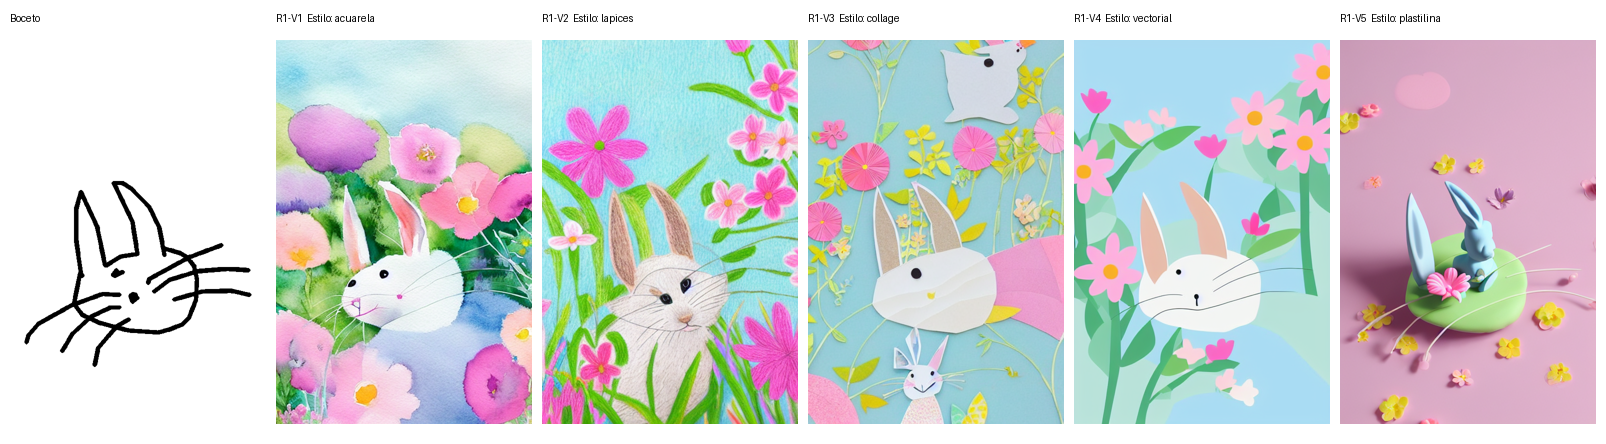
\includegraphics[width=0.78\textwidth]{assets/lamina_motor_a.png}\\[2pt]
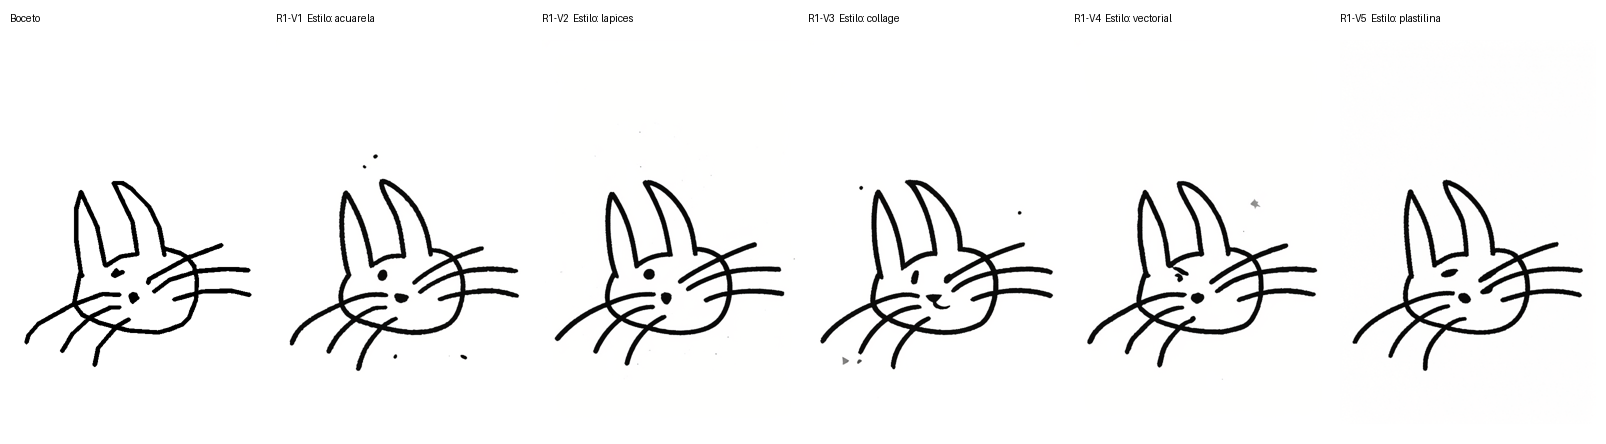
\includegraphics[width=0.78\textwidth]{assets/lamina_motor_b.png}
\caption{Una ronda con eje estilo a partir del mismo boceto: motor~A (arriba) y motor~B (abajo). El motor~A reinterpreta el dibujo en cada estilo; el motor~B casi lo copia y los cinco estilos apenas se distinguen.}\label{fig:motores}
\end{figure*}

\begin{figure}[t]
\centering
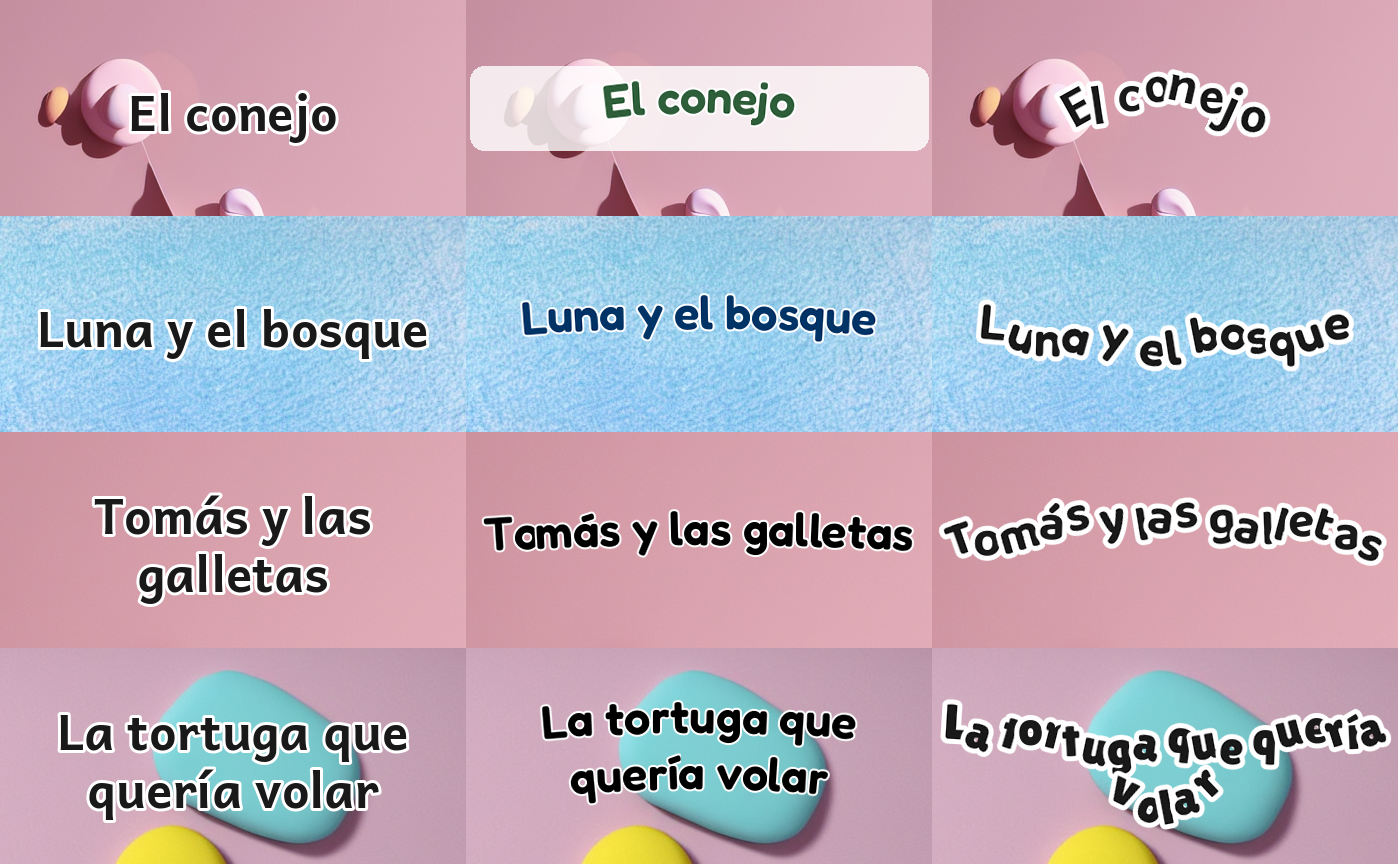
\includegraphics[width=0.72\columnwidth]{assets/muestras_titulos.png}
\caption{Títulos sobre portadas de E1: disposición por defecto (izquierda), agente tipográfico (centro) y deformaciones extremas (derecha). En ``El conejo'' el dibujo queda detrás de las letras y el OCR lo lee como texto, aunque a simple vista se lee bien.}\label{fig:titulos}
\end{figure}

\textbf{E2: planificador.} Con 500 usuarios simulados, la aceptación media de Thompson es 35.3, 34.9 y 43.0\,\% en las rondas 1 a 3, y la de la política aleatoria, 35.3, 34.7 y 34.8\,\%. La ventaja aparece en la ronda 3, cuando ya hay evidencia de dos rondas; en la ronda 2 no hay diferencia, porque tras una sola ronda hay apenas cinco decisiones. Antes de corregir la asignación de crédito (actualizar solo los parámetros que variaron en la ronda) la ventaja parecía mayor, pero era un artefacto: los valores que no cambiaban acumulaban evidencia en cada aceptación.

\textbf{E3: resúmenes.} Con 30 sesiones simuladas, Qwen2.5-7B superó el validador al primer intento en el 67\,\% (10\,\% de plantilla; 1.5 intentos, 40\,s) y Phi-3.5-mini en el 13\,\% (53\,\% de plantilla; 2.5 intentos, 72\,s); se recomienda Qwen. Un script que contrasta cada resumen con el registro de la sesión halló fieles 23 de los 27 resúmenes de Qwen (85\,\%) y 7 de los 14 de Phi (50\,\%). No evalúa la parte interpretativa (``prefiere colores cálidos'') y la revisión humana de los casos discrepantes fue parcial.

\textbf{Agente de historia.} Con las 30 historias en inglés y las 30 en español anotadas a mano por una persona, la precisión $\geq 90$\,\% \emph{no se cumple}. Con comparación estricta, Qwen2.5 alcanza 74\,\% en inglés y 62\,\% en español, y Phi-3.5, 71\,\% y 59\,\%; con comparación flexible (un elemento puede contener al otro, como ``big red ball'' y ``ball''), 80\,\% y 69\,\% (Qwen) y 73\,\% y 64\,\% (Phi). Los falsos positivos son en parte errores reales (``ball'' como personaje, elementos que la historia no dice) y en parte diferencias con la anotación (``mother'' frente a ``mom''). El prompt se ajustó tras una primera corrida sobre las mismas historias, por lo que no es una estimación independiente.

\textbf{Legibilidad del título.} En 100 portadas de E1 leídas con Tesseract (español), el error por carácter medio es 43.4\,\% por defecto, 17.6\,\% con el agente tipográfico y 81.8\,\% con deformaciones extremas (prueba de estrés); ninguno llega al 5\,\%. La mediana es 0\,\% y el 64--66\,\% de las portadas se lee con error de 5\,\% o menos: la media la suben títulos cortos (``Dino'') o con un dibujo detrás (``El conejo''), cuyas formas el OCR lee como letras (Figura~\ref{fig:titulos}). Una persona revisó a mano las 20 portadas peor leídas por el OCR y las leyó sin esfuerzo todas; es una comprobación de un solo anotador y no sustituye la prueba con usuarios.

\textbf{E5: seguridad y sesgo.} El filtro de texto bloqueó las 20 entradas que debían rechazarse y 1 de 5 legítimas (``Elsa'', un nombre con marca); las 5 evasiones con eufemismos pasaron. De las 45 portadas generadas, una persona juzgó aptas 42 y no aptas 3 (payaso tenebroso, fantasma triste, dragón con miedo a la oscuridad). CLIP con umbral 0.5 no detectó ninguna (probabilidades 0.04, 0.29 y 0.35); con 0.25 detecta 2 de 3 sin bloquear ninguna de las 42 aptas, y el umbral queda en 0.25, una calibración débil (3 casos, un boceto, motor A). Se generaron 200 portadas por motor sin filtro y una persona revisó a mano las 25 con probabilidad $\geq 0.15$: 10 no eran aptas (3 del motor~A y 7 del B, sobre todo dragones). Con 0.25 el filtro detecta 5 de esas 10 y bloquea 5 aptas (1.3\,\% de las 400); con 0.5 no detecta ninguna. No se revisaron las de probabilidad menor, así que la detección real puede ser menor. En las 100 portadas de una figura sin rasgos, una sola persona anotó 79 de género ambiguo, 17 femeninas y 4 masculinas, y tono de piel visible en 20 (17 claros, 3 medios, ninguno oscuro); el estilo vectorial muestra más rasgos humanos (8 de 20).

% =====================================================================
\section{Consideraciones éticas y guardrails}\label{sec:etica}
\textbf{Contenido apto para niños.} El público final son niños, a quienes UNICEF identifica como un grupo que requiere protección y diseño específico en sistemas de IA. El filtro de seguridad de Stable Diffusion solo apunta a contenido sexual e ignora la violencia y otros contenidos perturbadores, por lo que no basta por sí solo. Guardrails implementados:
(1)~filtro de la historia, la instrucción libre y el título con lista de bloqueo (violencia, contenido sexual, odio); los elementos que extrae el agente de historia pasan por el mismo filtro antes de llegar al prompt;
(2)~prompt negativo fijo con términos de violencia y miedo;
(3)~sobre cada salida, el filtro de seguridad de SD más una verificación \emph{zero-shot} con CLIP contra descriptores como ``scary'', ``blood'' o ``weapon'', con un umbral calibrado en E5;
(4)~si una salida se marca, se regenera con otra semilla (máximo dos veces) y, si persiste, se muestra una tarjeta vacía que explica el motivo; todo queda registrado.

\textbf{Protección de menores y privacidad.} Se detectan rostros con MediaPipe y se rechaza toda foto de una persona real, porque el sistema trabaja con dibujos. Si el boceto lo hizo un menor, se pide el permiso del tutor. Las imágenes se procesan en memoria y se eliminan al cerrar la sesión; el registro guarda solo su hash. Todos los modelos corren dentro de la sesión de Colab, así que ni la historia, ni el boceto, ni las decisiones se envían a servicios externos; aun así, la interfaz advierte no escribir datos personales en los comentarios.

\textbf{Imitación de estilos y personajes protegidos.} Los modelos de difusión pueden replicar fragmentos de sus datos de entrenamiento e imitar el estilo de artistas concretos. Por eso los estilos son técnicas genéricas (acuarela, collage), no nombres de ilustradores, y la lista de bloqueo rechaza nombres de ilustradores, estudios y personajes con marca. Se explica al usuario que la portada es un concepto, que su protección por derechos de autor depende de la contribución humana y que debe declarar el uso de IA si publica.

\textbf{Sesgos.} Los libros infantiles del siglo XX muestran una subrepresentación sistemática de personajes femeninos, y los recuentos anuales del CCBC documentan la baja representación de autores y personajes diversos. Los modelos texto--imagen, a su vez, amplifican estereotipos demográficos. La hipótesis es que, ante un personaje humano poco definido, el modelo asigne por defecto ciertos rasgos. Como mitigación, el prompt no añade género ni etnia salvo que el usuario los indique, y E5(b) mide la distribución resultante; si se encuentra un sesgo marcado, se reportará y se ofrecerá un parámetro explícito de personaje.

\textbf{Impacto.} Un sistema así puede abaratar la autopublicación y la educación, pero también desplazar encargos a ilustradores. Lo planteamos como herramienta de exploración previa al trabajo con un ilustrador, no como su reemplazo. La Tabla~\ref{tab:rie} resume los riesgos y sus mitigaciones.

\begin{table}[t]
\centering\scriptsize
\caption{Riesgos identificados y mitigación.}\label{tab:rie}
\begin{tabularx}{\columnwidth}{@{}L{2.3cm}X@{}}
\toprule
\textbf{Riesgo} & \textbf{Mitigación}\\
\midrule
Contenido no apto para niños & Lista de bloqueo, prompt negativo, filtro de SD y verificación con CLIP, regeneración y registro.\\
\filasep
Fotos de menores & Detección de rostros y rechazo; permiso del tutor para dibujos de menores.\\
\filasep
Imitación de artistas o personajes & Estilos genéricos; bloqueo de nombres; aviso sobre derechos de autor.\\
\filasep
Sesgo en personajes & Prompt neutro; medición en E5(b); parámetro explícito si es necesario.\\
\filasep
Resumen infiel del LLM & Validador, máximo dos reintentos, plantilla y anotación manual.\\
\filasep
Elementos inventados de la historia & Verificación contra el texto y confirmación del usuario.\\
\filasep
Fuga de un manuscrito inédito & Todos los modelos corren en la sesión; nada se envía fuera.\\
\filasep
Título ilegible o deformado & Renderizado determinista, límites de deformación, contraste WCAG y OCR.\\
\filasep
Memoria o tiempo de GPU insuficiente & Motor B (10 pasos); lote de 5; reanudación de los experimentos; Colab Pro de una integrante.\\
\filasep
Fatiga del usuario & Máximo tres rondas; eje único por ronda.\\
\filasep
Pocos participantes & Resultados descriptivos.\\
\bottomrule
\end{tabularx}
\end{table}

% =====================================================================
\section{Plan de trabajo}
El trabajo se reparte siguiendo las cinco etapas del enunciado, con una responsable por etapa y una carga similar para cada integrante (Tabla~\ref{tab:roles}). Cada responsable mide las métricas de su módulo; el trabajo de campo (entrevistas, anotación y estudio con usuarios), el video y la presentación se reparten entre todas. La Tabla~\ref{tab:plan} muestra el cronograma hasta la entrega final \pend{fecha de entrega final}.

\begin{table}[t]
\centering\scriptsize
\caption{Reparto por etapas del enunciado. Cada integrante asume cerca del 20\,\% del esfuerzo total.}\label{tab:roles}
\begin{tabularx}{\columnwidth}{@{}L{1.55cm}XL{1.75cm}@{}}
\toprule
\textbf{Etapa} & \textbf{Responsabilidades} & \textbf{Integrantes}\\
\midrule
1. Problema y diseño & Design thinking, objetivos, alcance y arquitectura & Andrea Coa\\
\filasep
2. Datos & Selección de datos, licencias, análisis exploratorio y preprocesamiento & Jimena Gurbillon\\
\filasep
3. Modelo generativo & Motores de generación, calibración y evaluación de las portadas & Maria Surco\\
\filasep
4. Interfaz & Interfaz, tipografía y registro de la sesión & Bihonda Epiquien\\
\filasep
5. Explicación y evaluación & Agentes, planificador y evaluación con usuarios & Nayeli Guzman\\
\bottomrule
\end{tabularx}
\end{table}

\begin{table}[t]
\centering\scriptsize
\caption{Cronograma hasta la entrega final.}\label{tab:plan}
\begin{tabularx}{\columnwidth}{@{}lXL{2.1cm}@{}}
\toprule
\textbf{Sem.} & \textbf{Actividades} & \textbf{Hito}\\
\midrule
1 & Entrevistas, mapa de empatía, proto-persona y POV; descarga de D1, D2 y D4 y revisión de licencias; análisis exploratorio y preprocesamiento; motores A y B con un boceto; prototipo en papel de la interfaz & POV, datos listos y primera ronda de 5 portadas\\
\filasep
2 & Anotación de 30 historias y guardrails de entrada; calibración de la fidelidad y los pasos; agente de historia y verificador; agente tipográfico y renderizador; guardrails de salida; registro JSON; planificador y E2 & Sistema de una ronda con guardrails\\
\filasep
3 & Rondas múltiples; agente con Qwen2.5 y Phi-3.5, validador; E1 y E5; prueba piloto con 2 usuarios & Sistema integrado\\
\filasep
4 & E3 y E4 con 10 participantes; análisis; informe final; video de 3\,min con un participante ajeno a la carrera; ensayo de la presentación de 6\,min & Informe, código y demostración\\
\bottomrule
\end{tabularx}
\end{table}

\textbf{Entregables.} (1)~Repositorio con módulos separados (\texttt{preprocess}, \texttt{engines}, \texttt{planner}, \texttt{guardrails}, \texttt{agent}, \texttt{app}), un cuaderno de Colab reproducible, semillas fijas e instrucciones de ejecución; (2)~informe de máximo diez páginas; (3)~figuras de arquitectura, ejemplos de portadas por ronda y capturas de la interacción; (4)~video y presentación en vivo que muestren las cinco variaciones, la aceptación o rechazo y el resumen final.

\section{Conclusiones}
Acotar el sistema a portadas de libros infantiles convierte la generación de variaciones en una decisión con sentido para el usuario: la portada parte del boceto y de la historia del usuario, cada propuesta cambia un parámetro conocido, las decisiones alimentan un planificador explícito y el resumen del agente se verifica contra el registro. Los dos motores cubren los niveles básico e intermedio; el agente tipográfico da al título un aspecto lúdico sin perder legibilidad, porque las letras las dibuja siempre un renderizador determinista; y los guardrails responden a un público infantil. Las métricas, umbrales y experimentos ya están definidos; la siguiente etapa los pone a prueba con la implementación.

{\scriptsize

}

\end{document}
